\documentclass[11pt]{article}
\usepackage{amsmath,amssymb,amsthm}
\usepackage{bm}
\usepackage{algorithm}
\usepackage{algpseudocode}
\usepackage{booktabs}
\usepackage{graphicx}
\usepackage{hyperref}
\usepackage[margin=2.3cm]{geometry}
\setlength{\tabcolsep}{4.5pt}
\usepackage[section]{placeins}

\newcommand{\vphi}{\bm{\phi}}
\newcommand{\vpsi}{\bm{\psi}}
\newcommand{\w}{\mathbf{w}}
\newcommand{\cS}{\mathcal S}
\newcommand{\cA}{\mathcal A}
\newcommand{\cR}{\mathcal R}
\newcommand{\cL}{\mathcal L}
\newcommand{\R}{\mathbb R}
\DeclareMathOperator*{\argmax}{arg\,max}
\newtheorem{theorem}{Theorem}
\newtheorem{proposition}{Proposition}
\newtheorem{lemma}{Lemma}
\newtheorem{corollary}{Corollary}
\theoremstyle{definition}
\newtheorem{definition}{Definition}

\title{Certified SF libraries for zero-shot planning in stochastic domains}
\author{}
\date{\today}

\begin{document}
\maketitle

\noindent\textbf{Question.} Given a set of successor features, is GPI over them $\epsilon$-optimal for every
weight, so that any new FSA task can be planned zero-shot? If not, which policy must be added, and how can it be
obtained without training it? We answer both with Bellman gaps only: no linear system is solved, every quantity
is built from the one-step SF backup, which has a sample-based (TD) counterpart.

%=====================================================================================================
\section{Setting}

\begin{itemize}
\item MDP: finite $\cS,\cA$; $P(s'\mid s,a)\ge0$, $\sum_{s'}P(s'\mid s,a)\le1$ (missing mass: episode ends);
$\vphi(s,a)\in\R^d_{\ge0}$ expected features; $\gamma\in(0,1)$. Weights $\w\in\R^d_{\ge0}$,
$\Delta=\{\w\ge0:\sum_iw_i=1\}$.
\item Policy $\pi:\cS\to\cA$. SF backup
$(T^\pi\vpsi)(s,a)=\vphi(s,a)+\gamma\sum_{s'}P(s'\mid s,a)\,\vpsi(s',\pi(s'))$; the action SFs $\vpsi^\pi$ are its
fixed point. $Q^\pi_\w(s,a)=\vpsi^\pi(s,a)^\top\w$, $V^\pi_\w(s)=Q^\pi_\w(s,\pi(s))$, $V^*_\w=\max_\pi V^\pi_\w$.
\item Library $L$: a finite set of policies with their action SFs. GPI estimate and GPI policy \cite{barreto17}:
\[
\hat Q^L_\w(s,a)=\max_{\pi\in L}\vpsi^\pi(s,a)^\top\w,\qquad \pi^G_\w(s)\in\argmax_a\hat Q^L_\w(s,a),\qquad
V^{\pi^G_\w}_\w\ge\max_a\hat Q^L_\w(\cdot,a).
\]
\item Relevant states $\cR$: the start state and the exits (SF-FSA-VI reads values and starts subtasks only there).
\item Weight region: a union of faces $\Omega=\bigcup_{F\in\mathcal F}\Omega_F$,
$\Omega_F=\{\w\in\Delta:\mathrm{supp}(\w)\subseteq F\}$. A class of FSA tasks fixes $\mathcal F$: an automaton state that
accepts the symbols $\Sigma'$ puts weight only on their exits, so states branching on $\le m$ symbols need the faces of
$m$ symbols; $\mathcal F=\{\{1..d\}\}$ covers every FSA.
\item SF-FSA-VI \cite{kuric}, zero-shot: each automaton state $u$ gets $\w(u)\in[0,1]^d$ with
$w_e(u)=1$ if exit $e$ ends the task, $w_e(u)=\max_a\hat Q^L_{\w(v)}(e,a)$ if it leads to $v$, $0$ otherwise
(reverse topological order); the agent executes $\pi^G_{\w(u)}$ in $u$.
\end{itemize}

%=====================================================================================================
\section{Solve-free primitives}

\paragraph{Evaluation.} $\vpsi_{k+1}=T^\pi\vpsi_k$ from any start $\vpsi_0$; $\|\vpsi_k-\vpsi^\pi\|_\infty\le
\frac{\gamma}{1-\gamma}\|\vpsi_k-\vpsi_{k-1}\|_\infty$. With samples: TD on stored transitions $(s,a,\vphi,s')$.
Cost unit: one \emph{sweep} = one backup of all $(s,a)$.

\paragraph{Bellman gap.} $g^\pi_\w(s)=\max_aQ^\pi_\w(s,a)-V^\pi_\w(s)\ge0$; read off the action-SF table.

\paragraph{Reachable layers.} $\cL_0(r)=\{r\}$, $\cL_{t+1}(r)=\{s':\exists s\in\cL_t(r),a,\ P(s'\mid s,a)>0\}$; they
become constant after some $t_0$.

\begin{proposition}[gap bound]\label{prop:gap}
For any $\pi$, $\w$, $r$:
\[
g^\pi_\w(r)\ \le\ V^*_\w(r)-V^\pi_\w(r)\ \le\ B^\pi_\w(r):=\textstyle\sum_{t\ge0}\gamma^t\max_{s\in\cL_t(r)}g^\pi_\w(s).
\]
More generally, for any $V:\cS\to\R$ with residual
$\rho(s)=\max_a[r_\w(s,a)+\gamma\sum_{s'}P(s'\mid s,a)V(s')]-V(s)$:\quad
$V^*_\w(r)-V(r)\le\sum_t\gamma^t\max_{\cL_t(r)}\rho^+$.
\end{proposition}
\begin{proof}
Upper: $V^*-V=(T^{\pi^*}V^*-T^{\pi^*}V)+(T^{\pi^*}V-V)\le\gamma P_{\pi^*}(V^*-V)+\rho$; iterate; row $r$ of
$P^t_{\pi^*}$ is a sub-probability on $\cL_t(r)$. With $V=V^\pi$, $\rho=g^\pi$. Lower: $V^*(r)\ge
\max_a[r_\w(r,a)+\gamma\sum P V^\pi]=V^\pi(r)+g^\pi(r)$.
\end{proof}

%=====================================================================================================
\section{The certificate}

\begin{definition}[records]
A record $(\w_q,\mathbf u_q)$, $\w_q\in\Omega_F$, $\mathbf u_q\in\R^{\cR}$, satisfies $u_q(r)\ge V^*_{\w_q}(r)$ for all
$r$. Any evaluated policy $\pi$ gives one: $u_q(r)=V^\pi_{\w_q}(r)+B^\pi_{\w_q}(r)$ (Proposition~\ref{prop:gap}).
\end{definition}

For a face $F$, $r\in\cR$ and $\w\in\Omega_F$ define (records restricted to $\Omega_F$)
\[
E_r(\w)=\max_{\pi\in L,\,a\in\cA}\vpsi^\pi(r,a)^\top\w,
\]
\[
U^F_r(\w)=\min\Big\{\textstyle\sum_q\lambda_qu_q(r):\ \sum_q\lambda_q\w_q=\w,\ \lambda\ge0,\ \w_q\in\Omega_F\Big\}.
\]
$E_r$ is convex and piecewise affine; its \emph{corners} $C^F_r$ are the vertices of its linearity regions in
$\Omega_F$ (the vertices of $\{\w\in\Omega_F:\vpsi^\pi(r,a)^\top\w\ge E_r(\w)\}$ over all $(\pi,a)$). $U^F_r$ is the lower
convex envelope of the records in $\Omega_F$.

\begin{theorem}[certificate]\label{thm:cert}
Let $\Gamma=\max_{F\in\mathcal F}\max_{r\in\cR}\max_{\mathbf c\in C^F_r}\,[U^F_r(\mathbf c)-E_r(\mathbf c)]$ (corners and
records of each face). Then for every $\w\in\R^d_{\ge0}$ with $\w/\|\w\|_1\in\Omega$ and every $r\in\cR$,
\[
V^*_\w(r)-V^{\pi^G_\w}_\w(r)\ \le\ V^*_\w(r)-\max_a\hat Q^L_\w(r,a)\ \le\ \Gamma\,\|\w\|_1 .
\]
\end{theorem}
\begin{proof}
First inequality: GPI \cite{barreto17}. $\max_a\hat Q^L_\w(r,a)=E_r(\w)$. $V^*_\w(r)$ is convex in $\w$ (maximum of
linear functions), so $V^*_\w(r)\le U_r(\w)$. On each linearity region of $E_r$, $U_r-E_r$ is convex, so its maximum
over the region is attained at a vertex; hence $\max_{\Omega_F}(U_r-E_r)=\max_{C_r}(U_r-E_r)\le\Gamma$. Both sides
are positively homogeneous of degree 1 in $\w$.
\end{proof}

\noindent The bound covers both what GPI achieves and what the planner believes (the estimate), at every
relevant state, for every weight of the face. It needs only the stored SFs at $\cR$ and the records.

\begin{corollary}[zero-shot FSA]\label{cor:fsa}
Assume one-hot exit features (so $\sum_i\psi^\pi_i(s)\le1$). For an acyclic task of depth $H$ (longest path from
$u_0$) whose weights $\w(u)$ lie in the certified face, with $m=\max_u\|\w(u)\|_1$, the zero-shot policy loses at
most $(H+1)^2\,m\,\Gamma$ with respect to the optimal policy of SF-FSA-VI.
\end{corollary}
\begin{proof}[Sketch]
Let $\delta_u=\|\w(u)-\w^*(u)\|_\infty$ and $\varepsilon_u$ the worst loss from $u$ at relevant states. Lipschitzness of
$V^*_\w$ in $\w$ (constant 1) and Theorem~\ref{thm:cert} give $\delta_u\le\max_v(\delta_v+m\Gamma)$ and
$\varepsilon_u\le\delta_u+m\Gamma+\max_v(\delta_v+m\Gamma+\varepsilon_v)$ over successors $v$; induction on depth.
\end{proof}

%=====================================================================================================
\section{Building a certified library}

$L$ is split into the \emph{base} $B$ (policies obtained by control) and \emph{compositions} (obtained by evaluating a
policy built from $L$). A corner $(\mathbf c,r)$ is \emph{closed} when $U_r(\mathbf c)-E_r(\mathbf c)\le\theta$
($\theta=10^{-9}$: exact mode).

\begin{algorithm}[H]
\caption{Certified library (CL)}
\begin{algorithmic}[1]
\Require face $F$, tolerance $\epsilon$
\State $B=L\gets\{\pi^*_{\mathbf e_i}:i\in F\}$ (control); records at the vertices
\Loop
  \State $(\mathbf c,r)\gets$ corner with the largest gap (lazy max-heap; gaps only decrease)
  \If{gap $\le\epsilon$} \Return $L$ \Comment{$\Gamma\le\epsilon$} \EndIf
  \State \textsc{free}: record $\mathbf u=\min\big(\min_{\pi\in L}[V^\pi_{\mathbf c}+B^\pi_{\mathbf c}],\ \hat V+\textstyle\sum_t\gamma^t\max_{\cL_t}\rho^+\big)$ with
  $\hat V=\max_a\hat Q^L_{\mathbf c}$ \Comment{stored SFs; 1 backup}
  \State \textbf{if} closed: \textbf{continue}
  \State \textsc{compose}: evaluate $\pi^G_{\mathbf c}$ (warm start $\hat Q^L$); \textbf{if} $B^{\pi^G}_{\mathbf c}(r)\le\theta$: add to $L$, record, \textbf{continue}
  \State \textsc{meta}: policy iteration restricted to $\{\pi(s):\pi\in B\}$; \textbf{if} certified: add to $L$, record, \textbf{continue}
  \State \textsc{learn}: policy iteration over $\cA$ from the best candidate (anytime: stop when certified); add to $B$ and $L$, record
\EndLoop
\end{algorithmic}
\end{algorithm}

\begin{proposition}
(i) After a corner is answered, its gap is at most $\theta$. (ii) Gaps never increase, so the largest gap is an
anytime certificate $\Gamma_t$ of the current library. (iii) A policy is trained only at a weight where neither the
stored SFs, nor GPI's policy, nor the metapolicy over $B$ is certified.
\end{proposition}

\paragraph{Sufficiency test.} Algorithm~1 without \textsc{learn}: a corner that no rung closes is kept open, and the
best composition is still added (it is a valid policy with known SFs). It returns the certificate of everything that
can be composed from a given base $B$, and the weights where $B$ is not certified.

\paragraph{Corners.} For $|F|=2$ the corners are breakpoints of an upper envelope of lines (exact). For $|F|\ge3$ every
point's linearity region $\{\w\in\Omega_F:(\vpsi-\vpsi')^\top\w\ge0\ \forall\vpsi'\}$ is enumerated (Chebyshev centre by
LP, vertices by halfspace intersection); points whose region has no interior are discarded. $U^F_r$ is evaluated
through the lower facets of the convex hull of the records (or by its LP).

\paragraph{Sample-based version.} Replace $P$ by the empirical model $\hat P$ of a replay buffer: TD on the buffer
converges to the same SFs. Theorem~\ref{thm:cert} then holds for $\hat P$; for $P$ an additional model-error term is
needed (Section~\ref{sec:exp}).

%=====================================================================================================
\section{What a certificate costs}\label{sec:cost}

\begin{proposition}[informal]
A certificate of the form of Theorem~\ref{thm:cert} needs, for every $\w\in\Omega$, an evaluated policy in $L$ whose value
is within $\Gamma$ of $V^*_\w$ at every $r$: $L$ must be a $\Gamma$-cover of $\Omega$, i.e.\ at least as large as a
$\Gamma$-CCS. Compositions replace \emph{training} (control) by \emph{evaluation} (prediction), not the number of
evaluated policies. Iterating compositions at one weight is policy iteration (GPI over $L\cup\{\pi^G\}$ is at least
the greedy step), so a base of the $d$ extreme policies always suffices in principle; the cost moves into evaluations.
\end{proposition}
\noindent In deterministic domains with exit features the GPI estimate is already exact ($E_r=V^*$), so every corner
is closed by \textsc{free} and no composition is needed.

%=====================================================================================================
\section{Experiments}\label{sec:exp}
All runs are exact in $P$ (no sampling) unless stated; costs are SF sweeps; ``trained'' counts control problems
(policy iteration over all actions), ``library'' all stored SFs; true losses are measured on held-out weights inside
the certified region (ground truth by policy iteration). Every run is one anytime run; a row is its state when
$\Gamma\le\epsilon$ is first certified.

\paragraph{Deterministic Office (sanity check).} With the $6$ extreme policies every corner of the full $6$-exit
simplex is closed by \textsc{free}: $\Gamma=5.7\cdot10^{-8}$ at all $7$ relevant states after $383$ corner checks, $684$
sweeps, no composition and no training. GPI over the extremes is certified optimal for every FSA, recovering the
known deterministic result.

\paragraph{Double slit} (Kuric et al.'s DoubleSlit, wind $\pm3$, $\gamma=0.9$; Table~\ref{tab:ds}, Figure~\ref{fig:ds}).
All methods reach the same certificates with libraries of about the same size; the certified library trains $11$
policies instead of $309$, at the compute of warm-started SFOLS plus $9$--$20\%$, and $37\times$ less than SFOLS learning
every policy from scratch. The sufficiency test (Table~\ref{tab:suff}) shows that compositions alone, from the $2$ extreme
policies, already reach an exact certificate. With an empirical model (Table~\ref{tab:sampled}) the certificate is
only valid for $\hat P$: the true loss exceeds it until $n\approx10^4$ samples per state-action.

\paragraph{Windy two-stage and Office} (Tables~\ref{tab:windy}--\ref{tab:office1}, Figures~\ref{fig:windy},
\ref{fig:office}). Every certified library plans every task of its class zero-shot with regret below $10^{-5}$ (windy
$6.7\cdot10^{-6}$, Office $p=0.1$ $2.7\cdot10^{-6}$). The $6$ extreme policies lose up to $1.2\%$ in windy, where the
first stage must hedge between the two slits; in Office with $p=0.1$ they are already near-optimal on tasks
($1.6\cdot10^{-5}$) but not on the whole class (worst loss $6.6\cdot10^{-4}$ against $9.9\cdot10^{-5}$ for the certified
library). In windy the \textsc{free} rung closes many corners, so the certified library is both smaller and cheaper than
SFOLS ($15$ policies and $2{,}865$ sweeps against $23$ and $4{,}032$ at $\epsilon=10^{-3}$). In Office \textsc{free}
almost never closes a corner: the three methods certify with libraries of the same size, only $24$ of $255$ policies are
trained, and the certified library costs $5\%$ more sweeps than warm-started SFOLS (failed composition attempts).

\paragraph{Office, $p=0.3$ (provisional, runs in progress).} Same task class, $\epsilon=2\cdot10^{-3}$. At the last
checkpoint all three runs certify $\Gamma=9.2\cdot10^{-3}$: certified library $176$ policies ($21$ trained,
$36{,}101$ sweeps), Certify-or-Grow $178$ ($22$, $35{,}326$), warm-started SFOLS $178$ ($178$, $33{,}697$). The
pattern of $p=0.1$ repeats: about $8\times$ fewer trained policies, the same library and $7\%$ more compute.

\begin{figure}[h]\centering
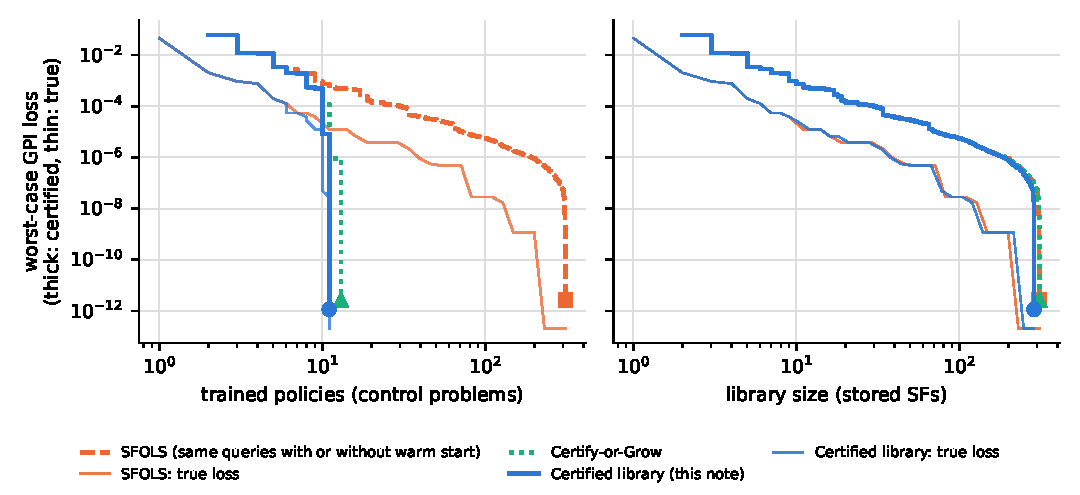
\includegraphics[width=0.9\linewidth]{figures/certlib_ds.pdf}
\caption{Double slit: anytime certificate (thick) and true worst-case loss (thin) against trained policies and
library size.}\label{fig:ds}
\end{figure}
\begin{figure}[h]\centering
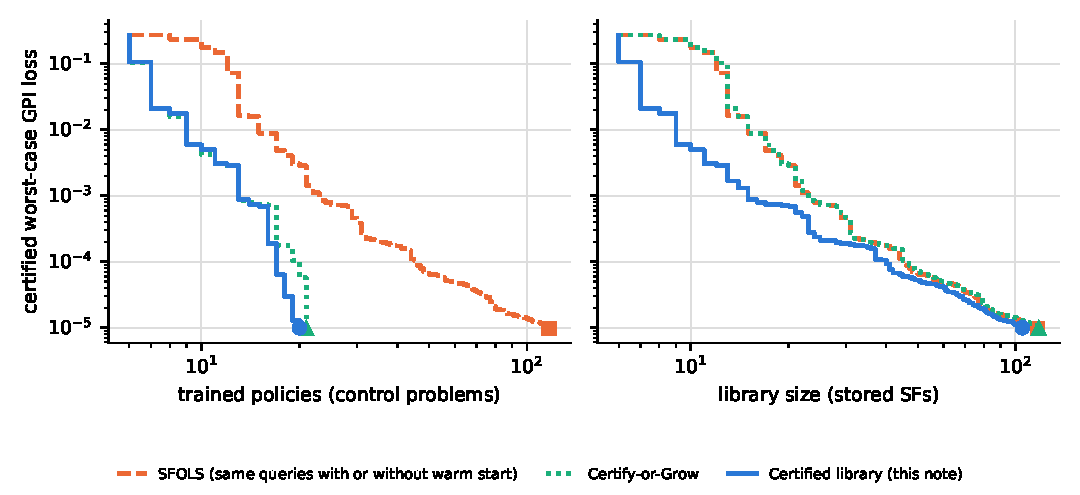
\includegraphics[width=0.9\linewidth]{figures/certlib_windy.pdf}
\caption{Windy two-stage: anytime certificate against trained policies and library size.}\label{fig:windy}
\end{figure}
\begin{figure}[h]\centering
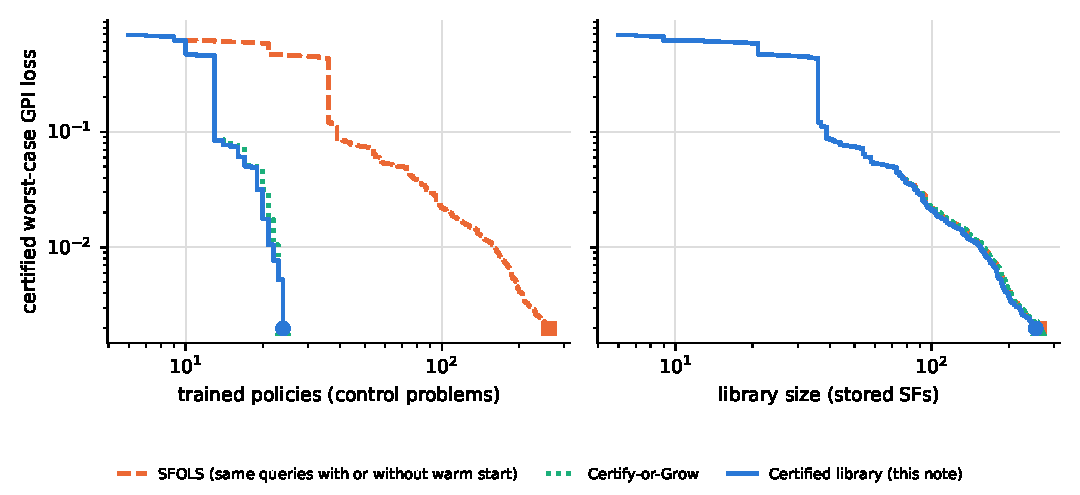
\includegraphics[width=0.9\linewidth]{figures/certlib_office1f2.pdf}
\caption{Office, $p=0.1$, three 4-exit faces: anytime certificate against trained policies and library size.}\label{fig:office}
\end{figure}

\begin{table}[h]\centering\small
\caption{Double slit (Kuric et al., wind $\pm3$, $\gamma=0.9$), weights on the whole simplex (the segment), relevant state = start. Each row is the state of one anytime run when $\Gamma\le\epsilon$ is first certified; true loss on 2001 weights.}\label{tab:ds}
\begin{tabular}{llrrrrr}
\toprule
$\epsilon$ & method & trained & library & sweeps & certified $\Gamma$ & true max loss\\
\midrule
$10^{-3}$ & SFOLS & 9 & 9 & 3933 & $9.6\cdot10^{-4}$ & $3.8\cdot10^{-5}$\\
$10^{-3}$ & SFOLS, warm start & 9 & 9 & 1250 & $9.6\cdot10^{-4}$ & $3.8\cdot10^{-5}$\\
$10^{-3}$ & Certify-or-Grow & 8 & 9 & 1408 & $9.6\cdot10^{-4}$ & $3.8\cdot10^{-5}$\\
$10^{-3}$ & Certified library & 8 & 9 & 1496 & $9.6\cdot10^{-4}$ & $3.8\cdot10^{-5}$\\
\midrule
$10^{-4}$ & SFOLS & 30 & 30 & 14134 & $9.5\cdot10^{-5}$ & $3.8\cdot10^{-6}$\\
$10^{-4}$ & SFOLS, warm start & 30 & 30 & 2185 & $9.5\cdot10^{-5}$ & $3.8\cdot10^{-6}$\\
$10^{-4}$ & Certify-or-Grow & 11 & 30 & 2396 & $9.5\cdot10^{-5}$ & $3.8\cdot10^{-6}$\\
$10^{-4}$ & Certified library & 10 & 30 & 2535 & $9.5\cdot10^{-5}$ & $3.8\cdot10^{-6}$\\
\midrule
$10^{-6}$ & SFOLS & 191 & 191 & 98762 & $9.8\cdot10^{-7}$ & $1.2\cdot10^{-9}$\\
$10^{-6}$ & SFOLS, warm start & 192 & 192 & 5269 & $9.8\cdot10^{-7}$ & $1.2\cdot10^{-9}$\\
$10^{-6}$ & Certify-or-Grow & 11 & 192 & 5480 & $9.8\cdot10^{-7}$ & $1.2\cdot10^{-9}$\\
$10^{-6}$ & Certified library & 11 & 186 & 5781 & $9.8\cdot10^{-7}$ & $1.2\cdot10^{-9}$\\
\midrule
exact & SFOLS & 310 & 310 & 274282 & $2.3\cdot10^{-11}$ & $2.1\cdot10^{-13}$\\
exact & SFOLS, warm start & 309 & 309 & 6788 & $2.6\cdot10^{-12}$ & $2.1\cdot10^{-13}$\\
exact & Certify-or-Grow & 13 & 310 & 7011 & $2.6\cdot10^{-12}$ & $2.1\cdot10^{-13}$\\
exact & Certified library & 11 & 287 & 7412 & $1.1\cdot10^{-12}$ & $2.1\cdot10^{-13}$\\

\bottomrule
\end{tabular}
\end{table}

\begin{table}[h]\centering\small
\caption{Sufficiency test on double slit: the base is the first $k$ trained policies of the certified-library run; afterwards only compositions (\textsc{free}, \textsc{compose}, \textsc{meta}), no training.}\label{tab:suff}
\begin{tabular}{rrrrrr}
\toprule
trained base & open corners & library & sweeps & certified $\Gamma$ & true max loss\\
\midrule
2 & 42 & 309 & 7784 & $2.0\cdot10^{-12}$ & $2.1\cdot10^{-13}$\\
4 & 27 & 299 & 7587 & $8.5\cdot10^{-11}$ & $2.1\cdot10^{-13}$\\
6 & 16 & 294 & 7161 & $2.0\cdot10^{-12}$ & $2.1\cdot10^{-13}$\\
8 & 5 & 290 & 6958 & $2.0\cdot10^{-12}$ & $2.1\cdot10^{-13}$\\
11 & 0 & 287 & 7051 & $2.0\cdot10^{-12}$ & $2.1\cdot10^{-13}$\\
\bottomrule
\end{tabular}
\end{table}

\begin{table}[h]\centering\small
\caption{Sample-based construction on double slit ($\epsilon=10^{-4}$): $n$ sampled outcomes per $(s,a)$ define $\hat P$; the library is certified on $\hat P$ and deployed on the true $P$.}\label{tab:sampled}
\begin{tabular}{rrrrr}
\toprule
$n$ & trained & library & $\Gamma$ on $\hat P$ & true max loss on $P$\\
\midrule
10 & 15 & 28 & $9.9\cdot10^{-5}$ & $1.3\cdot10^{-2}$\\
100 & 14 & 31 & $9.7\cdot10^{-5}$ & $1.6\cdot10^{-3}$\\
1000 & 11 & 29 & $9.9\cdot10^{-5}$ & $3.7\cdot10^{-4}$\\
10000 & 11 & 31 & $10^{-4}$ & $4.5\cdot10^{-5}$\\
\bottomrule
\end{tabular}
\end{table}

\begin{table}[h]\centering\small
\caption{Windy two-stage ($\gamma=0.95$): the faces of every two-stage task ($\{A,B\}$ and every pair of corridor exits); relevant = start and exits; regret over 60 tasks.}\label{tab:windy}
\begin{tabular}{llrrrrrr}
\toprule
$\epsilon$ & method & trained & library & sweeps & certified $\Gamma$ & true max loss & max task regret\\
\midrule
$10^{-3}$ & SFOLS & 23 & 23 & 7744 & $8.5\cdot10^{-4}$ & $1.2\cdot10^{-5}$ & 0 (0.00\%)\\
$10^{-3}$ & SFOLS, warm start & 23 & 23 & 4032 & $8.5\cdot10^{-4}$ & $1.2\cdot10^{-5}$ & 0 (0.00\%)\\
$10^{-3}$ & Certify-or-Grow & 13 & 23 & 4188 & $8.5\cdot10^{-4}$ & $1.2\cdot10^{-5}$ & 0 (0.00\%)\\
$10^{-3}$ & Certified library & 13 & 15 & 2865 & $8.8\cdot10^{-4}$ & $1.3\cdot10^{-5}$ & $6.7\cdot10^{-6}$ (0.00\%)\\
\midrule
$10^{-4}$ & SFOLS & 46 & 46 & 18808 & $8.8\cdot10^{-5}$ & $1.5\cdot10^{-7}$ & 0 (0.00\%)\\
$10^{-4}$ & SFOLS, warm start & 46 & 46 & 5007 & $8.8\cdot10^{-5}$ & $1.5\cdot10^{-7}$ & 0 (0.00\%)\\
$10^{-4}$ & Certify-or-Grow & 20 & 47 & 5442 & $8.8\cdot10^{-5}$ & $1.5\cdot10^{-7}$ & 0 (0.00\%)\\
$10^{-4}$ & Certified library & 17 & 40 & 4214 & $9.3\cdot10^{-5}$ & $8.4\cdot10^{-6}$ & $6.7\cdot10^{-6}$ (0.00\%)\\
\midrule
$10^{-5}$ & SFOLS & 117 & 117 & 53719 & $9.8\cdot10^{-6}$ & $1.1\cdot10^{-13}$ & 0 (0.00\%)\\
$10^{-5}$ & SFOLS, warm start & 117 & 117 & 6692 & $9.8\cdot10^{-6}$ & $1.1\cdot10^{-13}$ & 0 (0.00\%)\\
$10^{-5}$ & Certify-or-Grow & 21 & 118 & 7143 & $9.8\cdot10^{-6}$ & $1.1\cdot10^{-13}$ & 0 (0.00\%)\\
$10^{-5}$ & Certified library & 20 & 105 & 5869 & $10^{-5}$ & $1.1\cdot10^{-13}$ & 0 (0.00\%)\\
\midrule
-- & corners only & 6 & 6 & -- & -- & $3.4\cdot10^{-3}$ & $3.0\cdot10^{-3}$ (1.19\%)\\
\bottomrule
\end{tabular}
\end{table}

\begin{table}[h]\centering\small
\caption{Office with slip $p=0.1$ ($\gamma=0.99$): FSAs whose states branch on $\le2$ symbols (three 4-exit faces); relevant = start and exits; regret over 103 tasks.}\label{tab:office1}
\begin{tabular}{llrrrrrr}
\toprule
$\epsilon$ & method & trained & library & sweeps & certified $\Gamma$ & true max loss & max task regret\\
\midrule
$2.0\cdot10^{-2}$ & SFOLS, warm start & 108 & 108 & 19980 & $2.0\cdot10^{-2}$ & $3.5\cdot10^{-4}$ & $2.7\cdot10^{-6}$ (0.00\%)\\
$2.0\cdot10^{-2}$ & Certify-or-Grow & 21 & 108 & 20618 & $2.0\cdot10^{-2}$ & $3.5\cdot10^{-4}$ & $2.7\cdot10^{-6}$ (0.00\%)\\
$2.0\cdot10^{-2}$ & Certified library & 20 & 103 & 21016 & $2.0\cdot10^{-2}$ & $3.5\cdot10^{-4}$ & $2.7\cdot10^{-6}$ (0.00\%)\\
\midrule
$10^{-2}$ & SFOLS, warm start & 161 & 161 & 22746 & $9.8\cdot10^{-3}$ & $1.8\cdot10^{-4}$ & $2.7\cdot10^{-6}$ (0.00\%)\\
$10^{-2}$ & Certify-or-Grow & 23 & 161 & 23421 & $9.8\cdot10^{-3}$ & $1.8\cdot10^{-4}$ & $2.7\cdot10^{-6}$ (0.00\%)\\
$10^{-2}$ & Certified library & 22 & 155 & 23910 & $9.8\cdot10^{-3}$ & $1.8\cdot10^{-4}$ & $2.7\cdot10^{-6}$ (0.00\%)\\
\midrule
$5.0\cdot10^{-3}$ & SFOLS, warm start & 195 & 195 & 24438 & $4.8\cdot10^{-3}$ & $1.8\cdot10^{-4}$ & $2.7\cdot10^{-6}$ (0.00\%)\\
$5.0\cdot10^{-3}$ & Certify-or-Grow & 24 & 195 & 25144 & $4.8\cdot10^{-3}$ & $1.8\cdot10^{-4}$ & $2.7\cdot10^{-6}$ (0.00\%)\\
$5.0\cdot10^{-3}$ & Certified library & 24 & 188 & 25769 & $4.8\cdot10^{-3}$ & $1.8\cdot10^{-4}$ & $2.7\cdot10^{-6}$ (0.00\%)\\
\midrule
$2.0\cdot10^{-3}$ & SFOLS, warm start & 262 & 262 & 27848 & $2.0\cdot10^{-3}$ & $9.9\cdot10^{-5}$ & $2.7\cdot10^{-6}$ (0.00\%)\\
$2.0\cdot10^{-3}$ & Certify-or-Grow & 24 & 262 & 28554 & $2.0\cdot10^{-3}$ & $9.9\cdot10^{-5}$ & $2.7\cdot10^{-6}$ (0.00\%)\\
$2.0\cdot10^{-3}$ & Certified library & 24 & 255 & 29258 & $2.0\cdot10^{-3}$ & $9.9\cdot10^{-5}$ & $2.7\cdot10^{-6}$ (0.00\%)\\
\midrule
-- & corners only & 6 & 6 & -- & -- & $6.6\cdot10^{-4}$ & $1.6\cdot10^{-5}$ (0.00\%)\\
\bottomrule
\end{tabular}
\end{table}

% no stops for office3f2


%=====================================================================================================
\section{Assessment}
\begin{itemize}
\item \textbf{What is certified.} Theorem~\ref{thm:cert} bounds, for every weight of a face union and every relevant
state, both GPI's loss and the planner's error, from stored SFs and Bellman gaps only; Corollary~\ref{cor:fsa} turns it
into a zero-shot bound for every FSA of the class. The bound is valid but conservative (true losses are $20$--$800\times$
below $\Gamma$; task regrets lower still).
\item \textbf{Deterministic domains.} The $d$ extreme policies are certified exactly optimal with no composition and a
few hundred backups (Office).
\item \textbf{Stochastic domains.} Training drops to the extremes plus a few policies (or only the extremes, if
compositions are iterated); evaluations do not drop: the library has the size of an $\epsilon$-CCS
(Section~\ref{sec:cost}), and total compute is that of warm-started SFOLS plus $5$--$20\%$, except where \textsc{free}
closes corners (windy: $12$--$29\%$ less).
\item \textbf{Model-free.} With an empirical model the certificate holds for $\hat P$ only; the true loss can exceed it
by the model error, so a rigorous model-free certificate needs confidence terms.
\item \textbf{Scaling.} Corner enumeration is exact and cheap on edges, affordable on 4-exit faces, and expensive on the
full 6-exit simplex (tens of thousands of corners per relevant state).
\end{itemize}

\begin{thebibliography}{9}
\bibitem{kuric} D.~Kuric, G.~Infante, V.~G\'omez, A.~Jonsson, H.~van~Hoof. Planning with a learned policy
basis to optimally solve complex tasks. ICAPS 2024.
\bibitem{barreto17} A.~Barreto et al. Successor features for transfer in reinforcement learning. NeurIPS 2017.
\bibitem{alegre22} L.~N.~Alegre, A.~Bazzan, B.~C.~da~Silva. Optimistic linear support and successor features
as a basis for optimal policy transfer. ICML 2022.
\end{thebibliography}
\end{document}
